\section{hdass\-Clock Class Reference}
\label{classhdassClock}\index{hdassClock@{hdassClock}}
{\tt \#include $<$hdassclock.h$>$}

Inheritance diagram for hdass\-Clock:\begin{figure}[H]
\begin{center}
\leavevmode
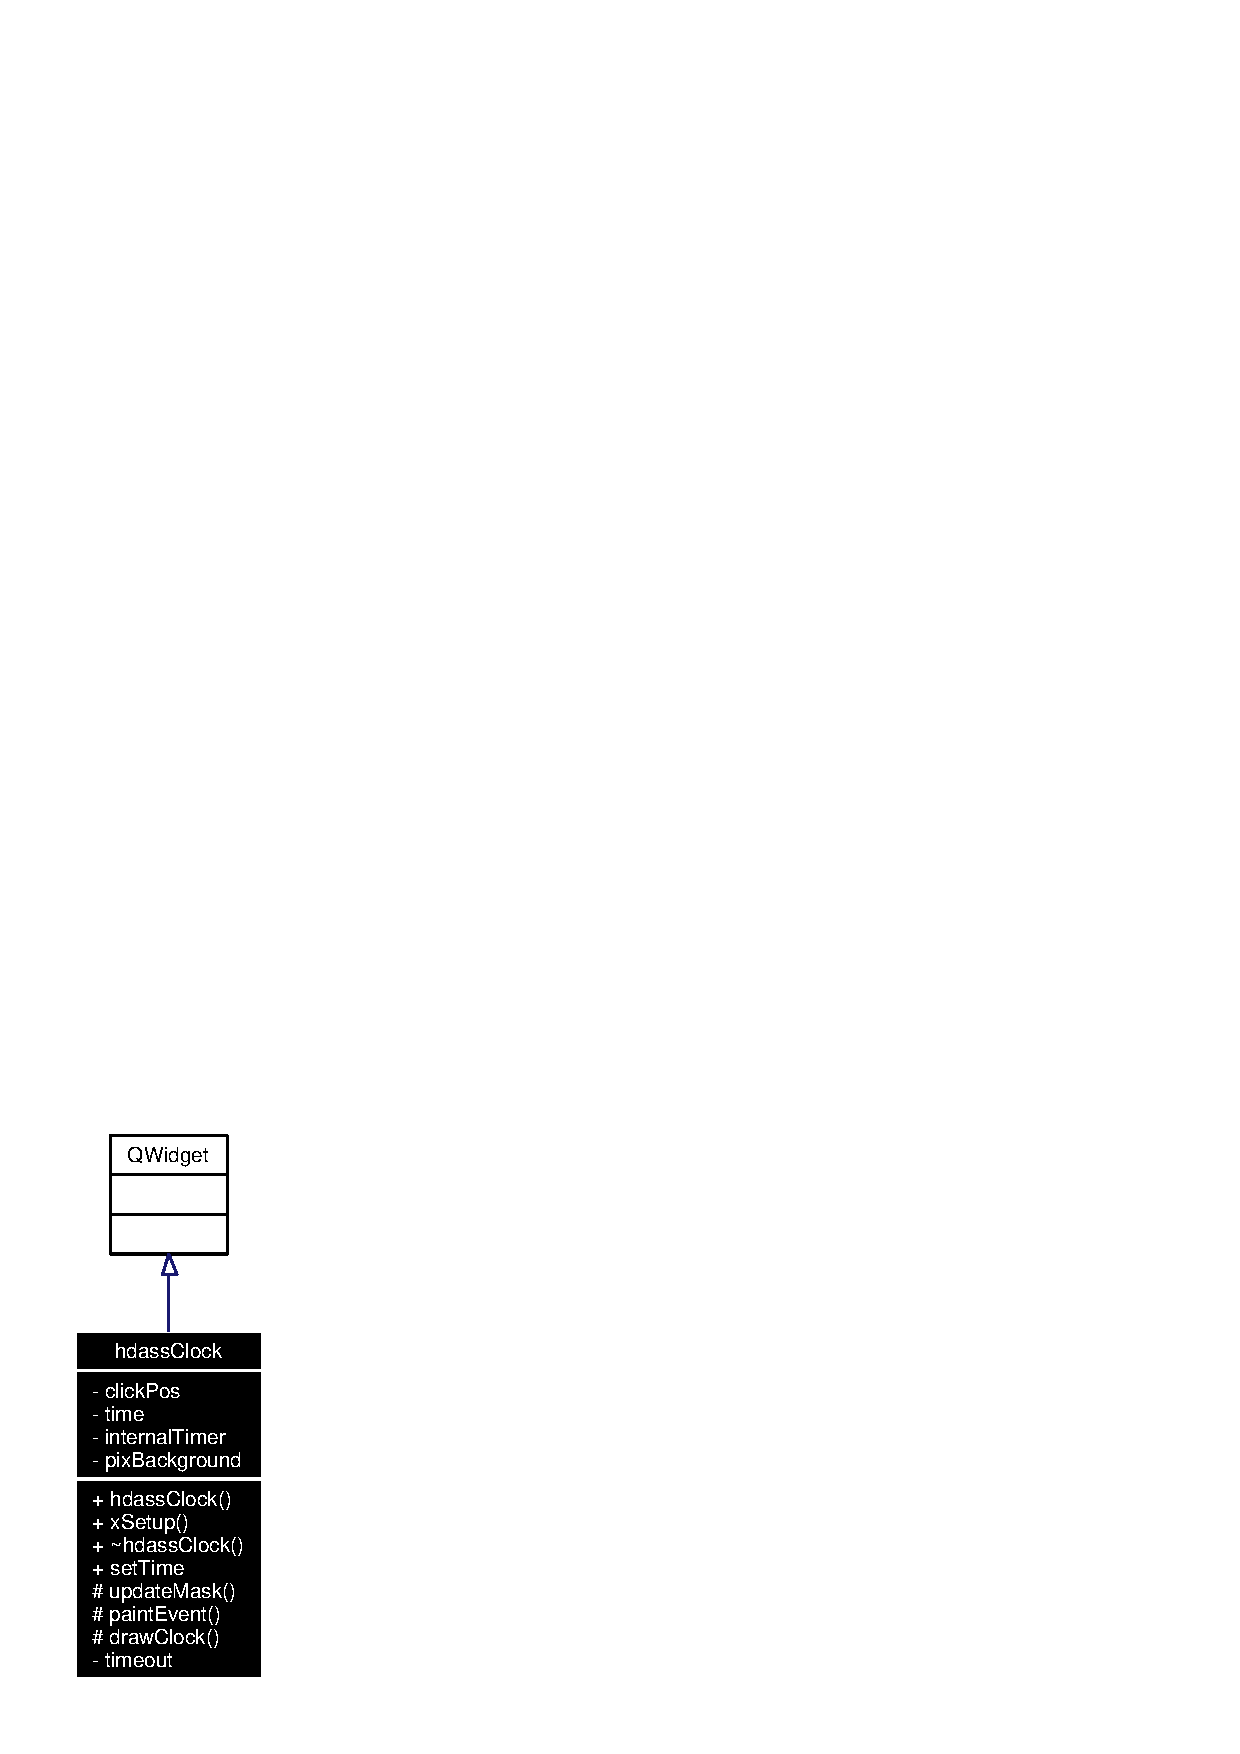
\includegraphics[width=63pt]{classhdassClock__inherit__graph}
\end{center}
\end{figure}
Collaboration diagram for hdass\-Clock:\begin{figure}[H]
\begin{center}
\leavevmode
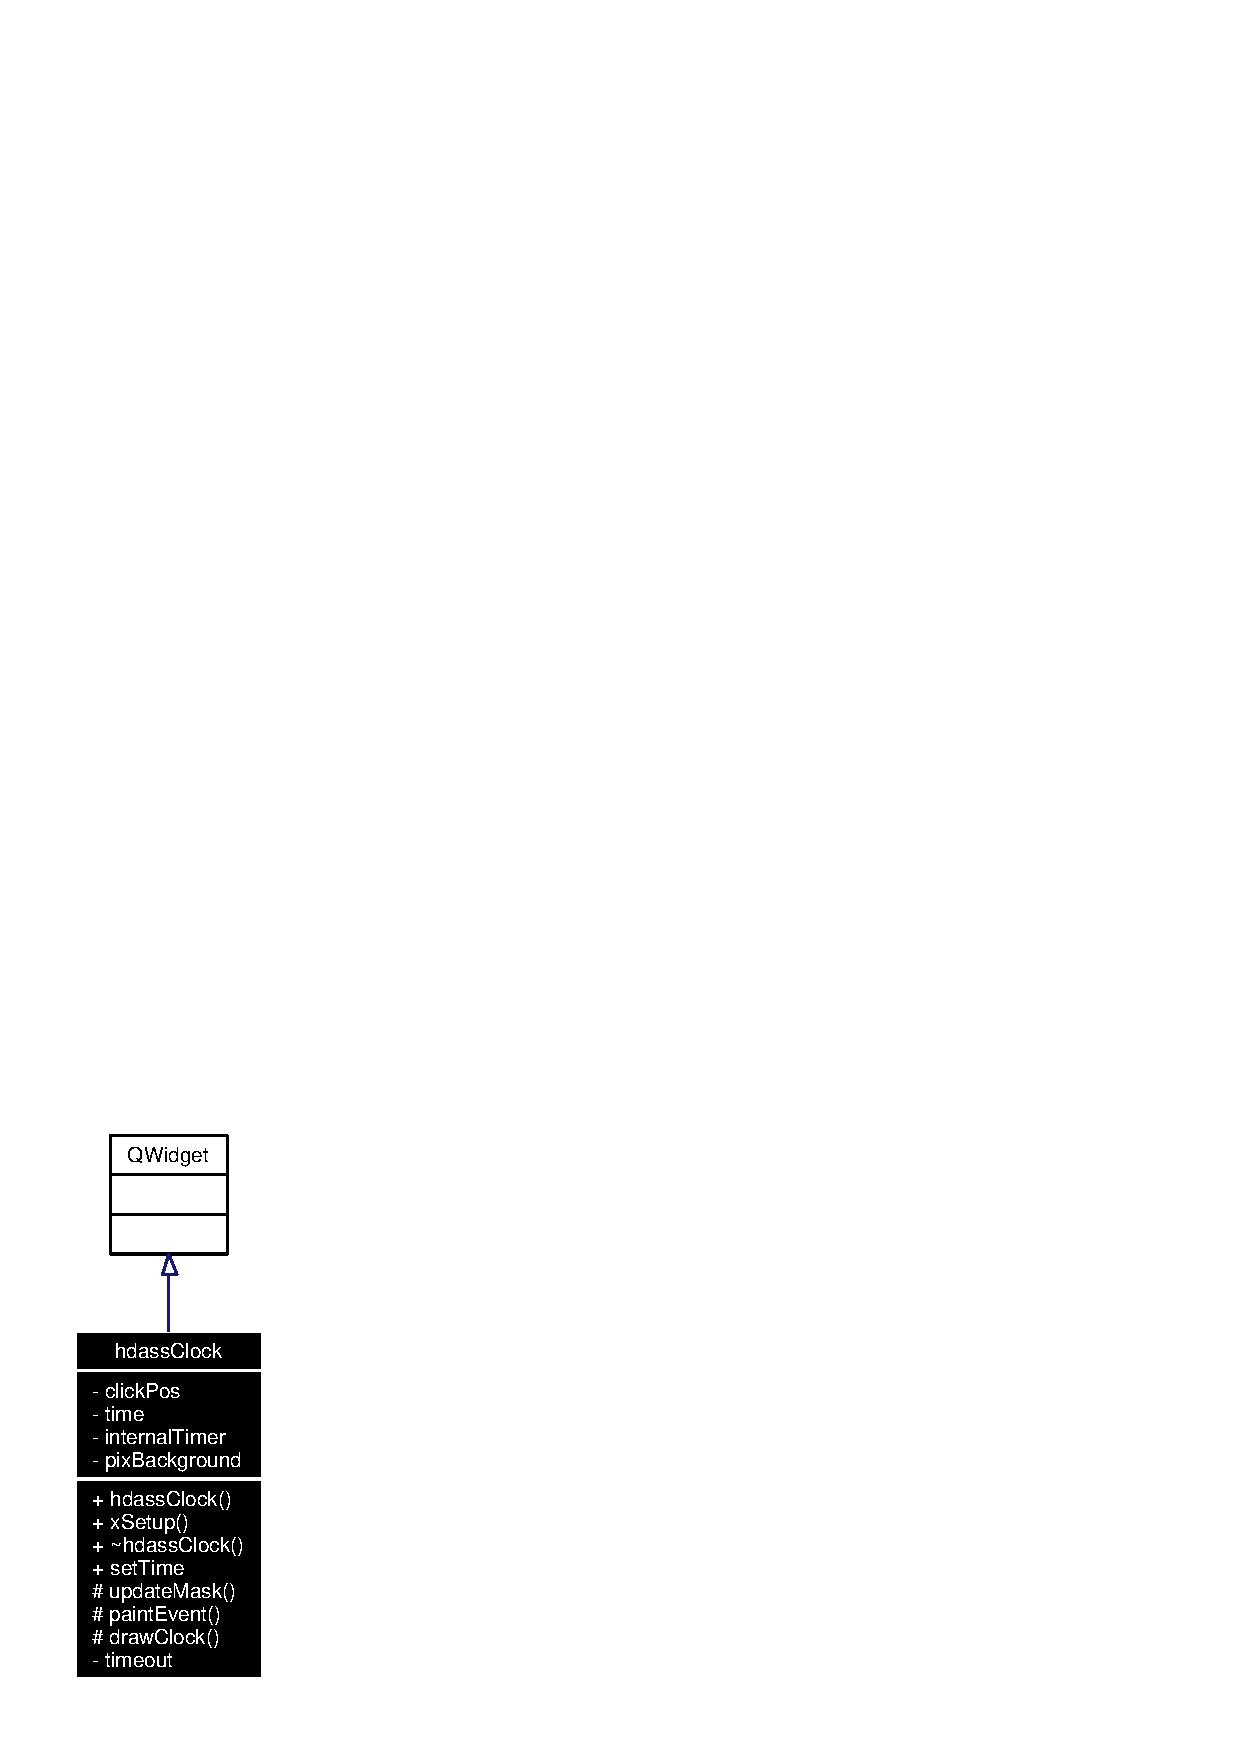
\includegraphics[width=63pt]{classhdassClock__coll__graph}
\end{center}
\end{figure}
\subsection*{Public Slots}
\begin{CompactItemize}
\item 
void {\bf set\-Time} (const QTime \&t)
\end{CompactItemize}
\subsection*{Public Member Functions}
\begin{CompactItemize}
\item 
{\bf hdass\-Clock} ({\bf QWidget} $\ast$parent=0, const char $\ast$name=0)
\item 
void {\bf x\-Setup} ()
\item 
{\bf $\sim$hdass\-Clock} ()
\end{CompactItemize}
\subsection*{Protected Member Functions}
\begin{CompactItemize}
\item 
void {\bf update\-Mask} ()
\item 
void {\bf paint\-Event} (QPaint\-Event $\ast$)
\item 
void {\bf draw\-Clock} (QPainter $\ast$)
\end{CompactItemize}
\subsection*{Private Slots}
\begin{CompactItemize}
\item 
void {\bf timeout} ()
\end{CompactItemize}
\subsection*{Private Attributes}
\begin{CompactItemize}
\item 
QPoint {\bf click\-Pos}
\item 
QTime {\bf time}
\item 
QTimer $\ast$ {\bf internal\-Timer}
\item 
QPixmap {\bf pix\-Background}
\end{CompactItemize}


\subsection{Constructor \& Destructor Documentation}
\index{hdassClock@{hdass\-Clock}!hdassClock@{hdassClock}}
\index{hdassClock@{hdassClock}!hdassClock@{hdass\-Clock}}
\subsubsection{\setlength{\rightskip}{0pt plus 5cm}hdass\-Clock::hdass\-Clock ({\bf QWidget} $\ast$ {\em parent} = 0, const char $\ast$ {\em name} = 0)}\label{classhdassClock_hdassClocka0}




Definition at line 24 of file hdassclock.cpp.

References x\-Setup().



\footnotesize\begin{verbatim}25  : QWidget(parent, name)
26 {
27    xSetup();
28 }
\end{verbatim}\normalsize 


Here is the call graph for this function:\begin{figure}[H]
\begin{center}
\leavevmode
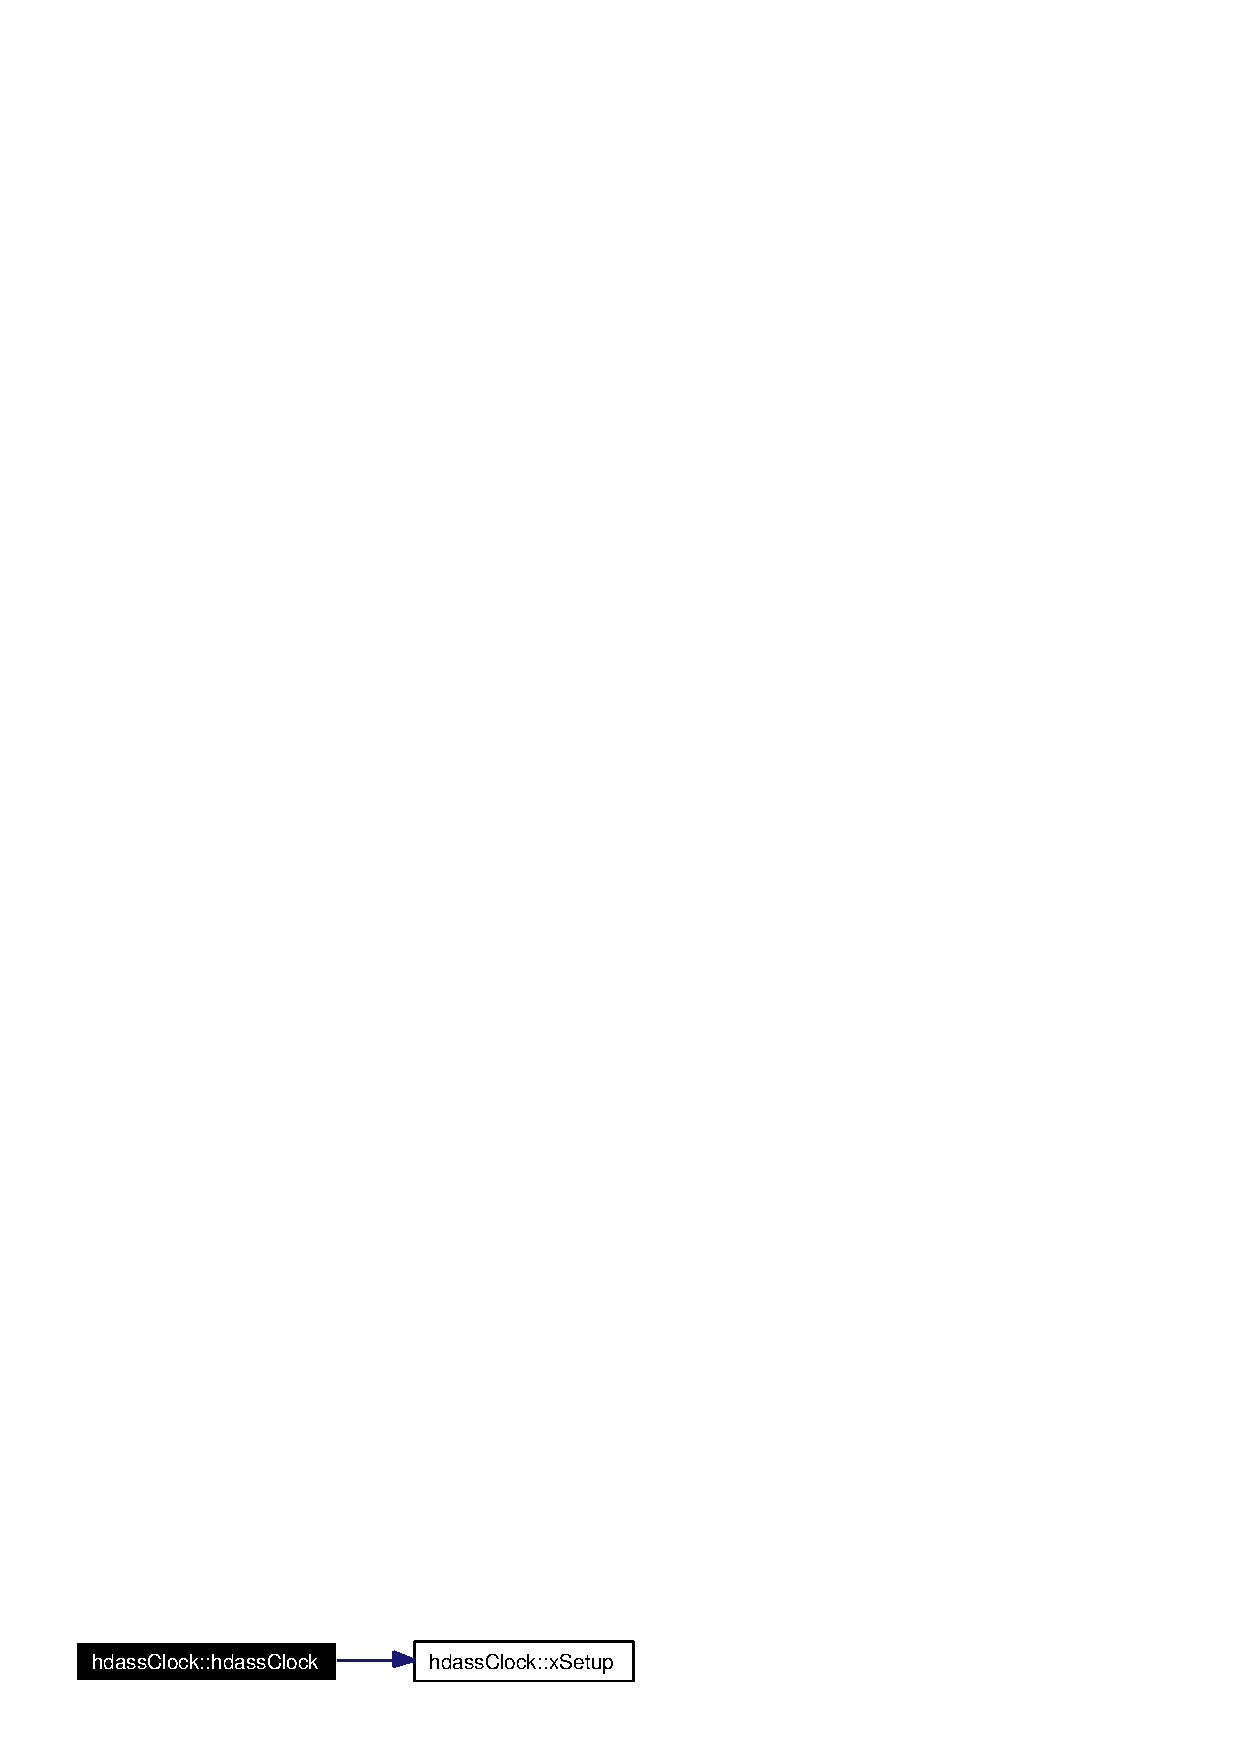
\includegraphics[width=152pt]{classhdassClock_hdassClocka0_cgraph}
\end{center}
\end{figure}
\index{hdassClock@{hdass\-Clock}!~hdassClock@{$\sim$hdassClock}}
\index{~hdassClock@{$\sim$hdassClock}!hdassClock@{hdass\-Clock}}
\subsubsection{\setlength{\rightskip}{0pt plus 5cm}hdass\-Clock::$\sim${\bf hdass\-Clock} ()}\label{classhdassClock_hdassClocka2}




Definition at line 31 of file hdassclock.cpp.



\footnotesize\begin{verbatim}32 {
33 
34 }
\end{verbatim}\normalsize 


\subsection{Member Function Documentation}
\index{hdassClock@{hdass\-Clock}!drawClock@{drawClock}}
\index{drawClock@{drawClock}!hdassClock@{hdass\-Clock}}
\subsubsection{\setlength{\rightskip}{0pt plus 5cm}void hdass\-Clock::draw\-Clock (QPainter $\ast$)\hspace{0.3cm}{\tt  [protected]}}\label{classhdassClock_hdassClockb2}




Definition at line 100 of file hdassclock.cpp.

References time.

Referenced by paint\-Event(), and update\-Mask().



\footnotesize\begin{verbatim}101 {
102     paint->setPen(Qt::white);
103     paint->save();
104     
105     paint->setWindow( -500,-500, 1000,1000 );
106 
107     QRect v = paint->viewport();
108     int d = QMIN( v.width(), v.height() );
109     paint->setViewport( v.left() + (v.width()-d)/2,v.top() + (v.height()-d)/2, d, d );
110     QPointArray pts;
111 
112     paint->save();
113     
114     paint->rotate( 30*(time.hour()%12-3) + time.minute()/2 ); 
115     QPixmap hr;
116     hr.load("/root/kde_application/hdass08/skin/hdassClockArrowHr.png"); 
117     paint->drawPixmap(0,(hr.height()/2)-100,hr);
118     paint->restore();
119 
120     paint->save();
121     paint->rotate( (time.minute()-15)*6 );
122     QPixmap min;
123     min.load("/root/kde_application/hdass08/skin/hdassClockArrowMin.png");
124     paint->drawPixmap(0,(min.height()/2)-90,min);
125     paint->restore();
126 }
\end{verbatim}\normalsize 
\index{hdassClock@{hdass\-Clock}!paintEvent@{paintEvent}}
\index{paintEvent@{paintEvent}!hdassClock@{hdass\-Clock}}
\subsubsection{\setlength{\rightskip}{0pt plus 5cm}void hdass\-Clock::paint\-Event (QPaint\-Event $\ast$)\hspace{0.3cm}{\tt  [protected]}}\label{classhdassClock_hdassClockb1}




Definition at line 73 of file hdassclock.cpp.

References draw\-Clock().



\footnotesize\begin{verbatim}74 {
75     if ( autoMask() )
76         return;
77     QPainter paint( this );
78     paint.setBrush( colorGroup().foreground() );
79     drawClock( &paint );
80 }
\end{verbatim}\normalsize 


Here is the call graph for this function:\begin{figure}[H]
\begin{center}
\leavevmode
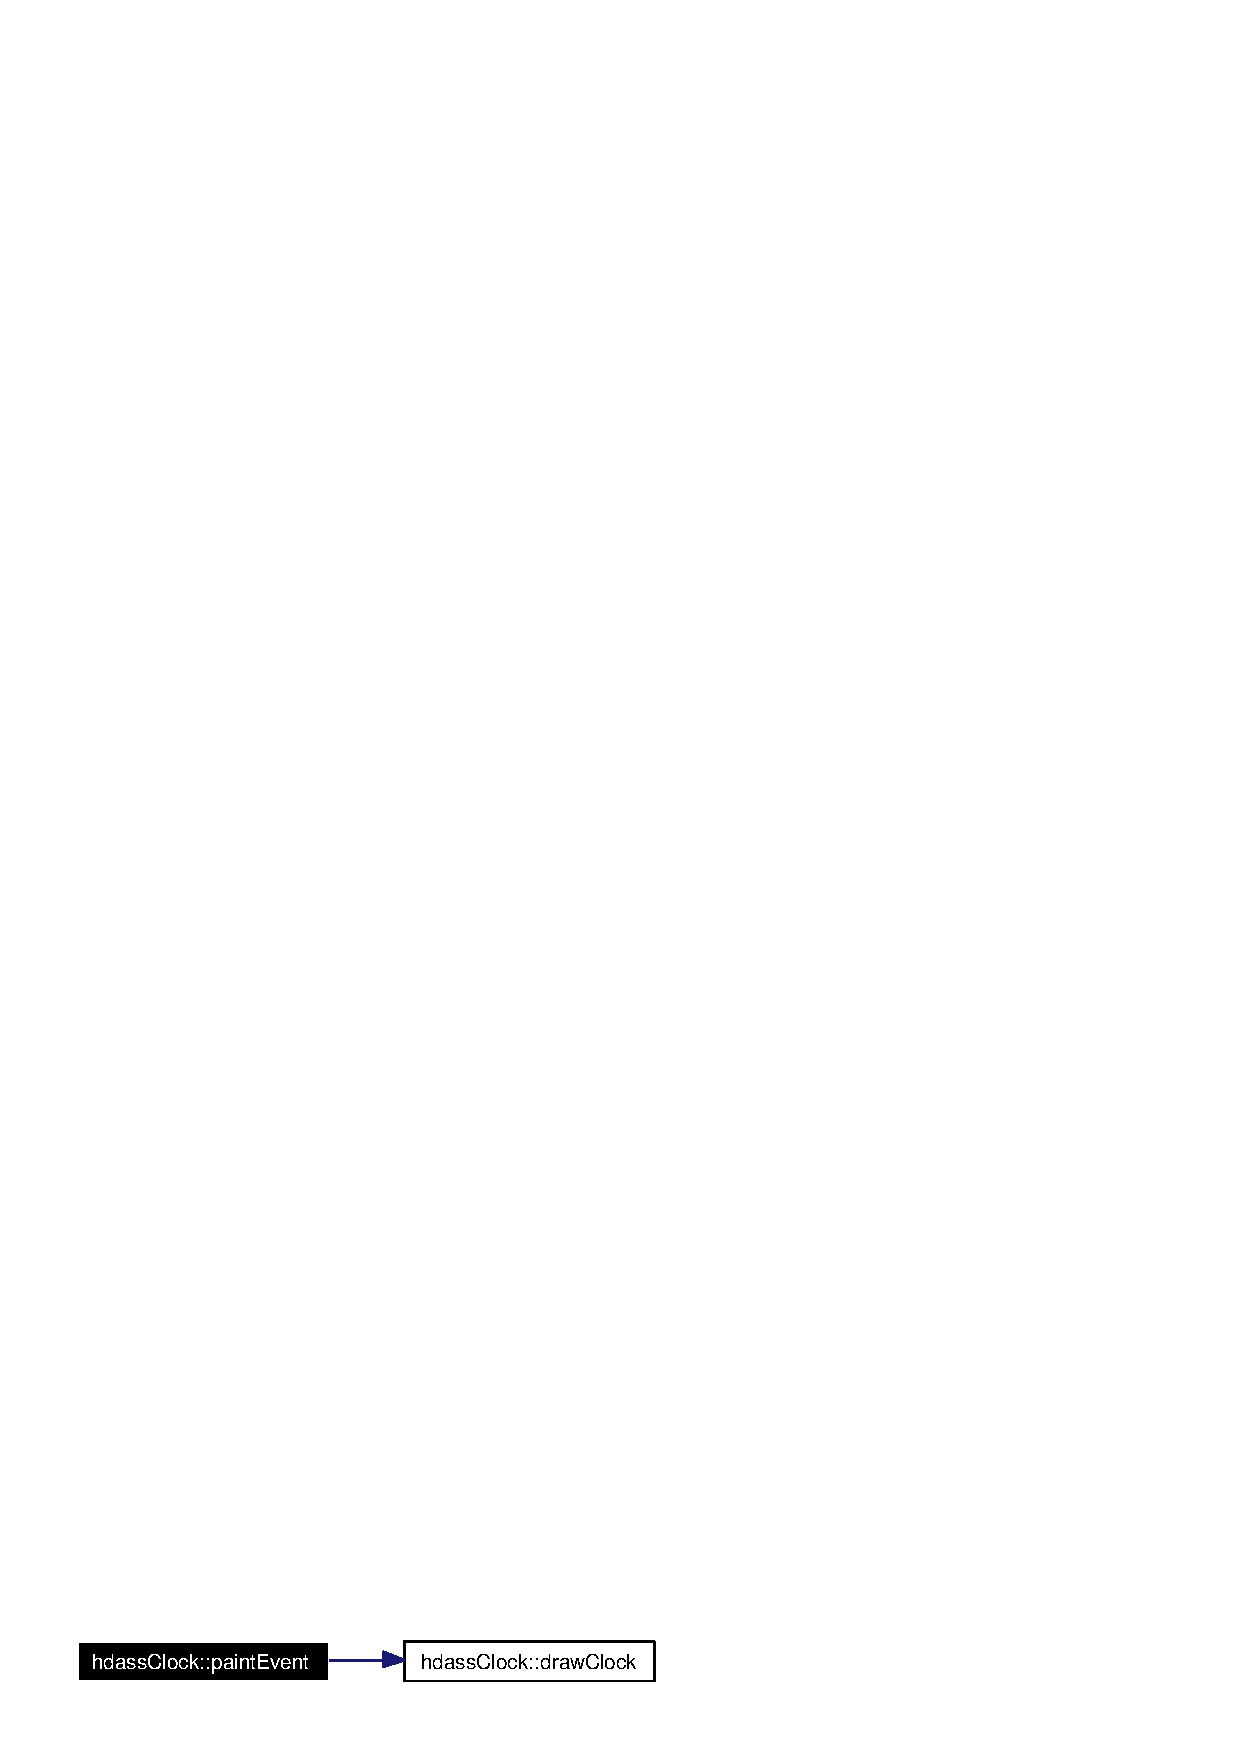
\includegraphics[width=157pt]{classhdassClock_hdassClockb1_cgraph}
\end{center}
\end{figure}
\index{hdassClock@{hdass\-Clock}!setTime@{setTime}}
\index{setTime@{setTime}!hdassClock@{hdass\-Clock}}
\subsubsection{\setlength{\rightskip}{0pt plus 5cm}void hdass\-Clock::set\-Time (const QTime \& {\em t})\hspace{0.3cm}{\tt  [slot]}}\label{classhdassClock_hdassClocki0}




Definition at line 49 of file hdassclock.cpp.

References internal\-Timer, time, timeout(), and update\-Mask().



\footnotesize\begin{verbatim}50 {
51   time = t;
52     disconnect( internalTimer, SIGNAL(timeout()), this, SLOT(timeout()) );
53     if (autoMask())
54         updateMask();
55     else
56         update();
57  
58 }
\end{verbatim}\normalsize 
\index{hdassClock@{hdass\-Clock}!timeout@{timeout}}
\index{timeout@{timeout}!hdassClock@{hdass\-Clock}}
\subsubsection{\setlength{\rightskip}{0pt plus 5cm}void hdass\-Clock::timeout ()\hspace{0.3cm}{\tt  [private, slot]}}\label{classhdassClock_hdassClockk0}




Definition at line 60 of file hdassclock.cpp.

References time, and update\-Mask().

Referenced by set\-Time(), and x\-Setup().



\footnotesize\begin{verbatim}61 {
62     QTime old_time = time;
63     time = QTime::currentTime();
64     if ( old_time.minute() != time.minute() 
65         || old_time.hour() != time.hour() ) {   // minute or hour has changed
66         if (autoMask())
67             updateMask();
68         else
69             update();
70     }
71 }
\end{verbatim}\normalsize 
\index{hdassClock@{hdass\-Clock}!updateMask@{updateMask}}
\index{updateMask@{updateMask}!hdassClock@{hdass\-Clock}}
\subsubsection{\setlength{\rightskip}{0pt plus 5cm}void hdass\-Clock::update\-Mask ()\hspace{0.3cm}{\tt  [protected]}}\label{classhdassClock_hdassClockb0}




Definition at line 82 of file hdassclock.cpp.

References draw\-Clock().

Referenced by set\-Time(), and timeout().



\footnotesize\begin{verbatim}83 {
84    QBitmap bm( size() );
85     //bm.fill( color0 );                        //transparent
86 
87     QPainter paint;
88     paint.begin( &bm, this );
89     QBrush brush=QBrush(white);
90     brush.setStyle(SolidPattern); 
91     paint.setBrush( brush );            // use non-transparent color
92     paint.setPen(color1);
93 
94     drawClock( &paint );
95 
96     paint.end();
97     setMask( bm );
98 }
\end{verbatim}\normalsize 


Here is the call graph for this function:\begin{figure}[H]
\begin{center}
\leavevmode
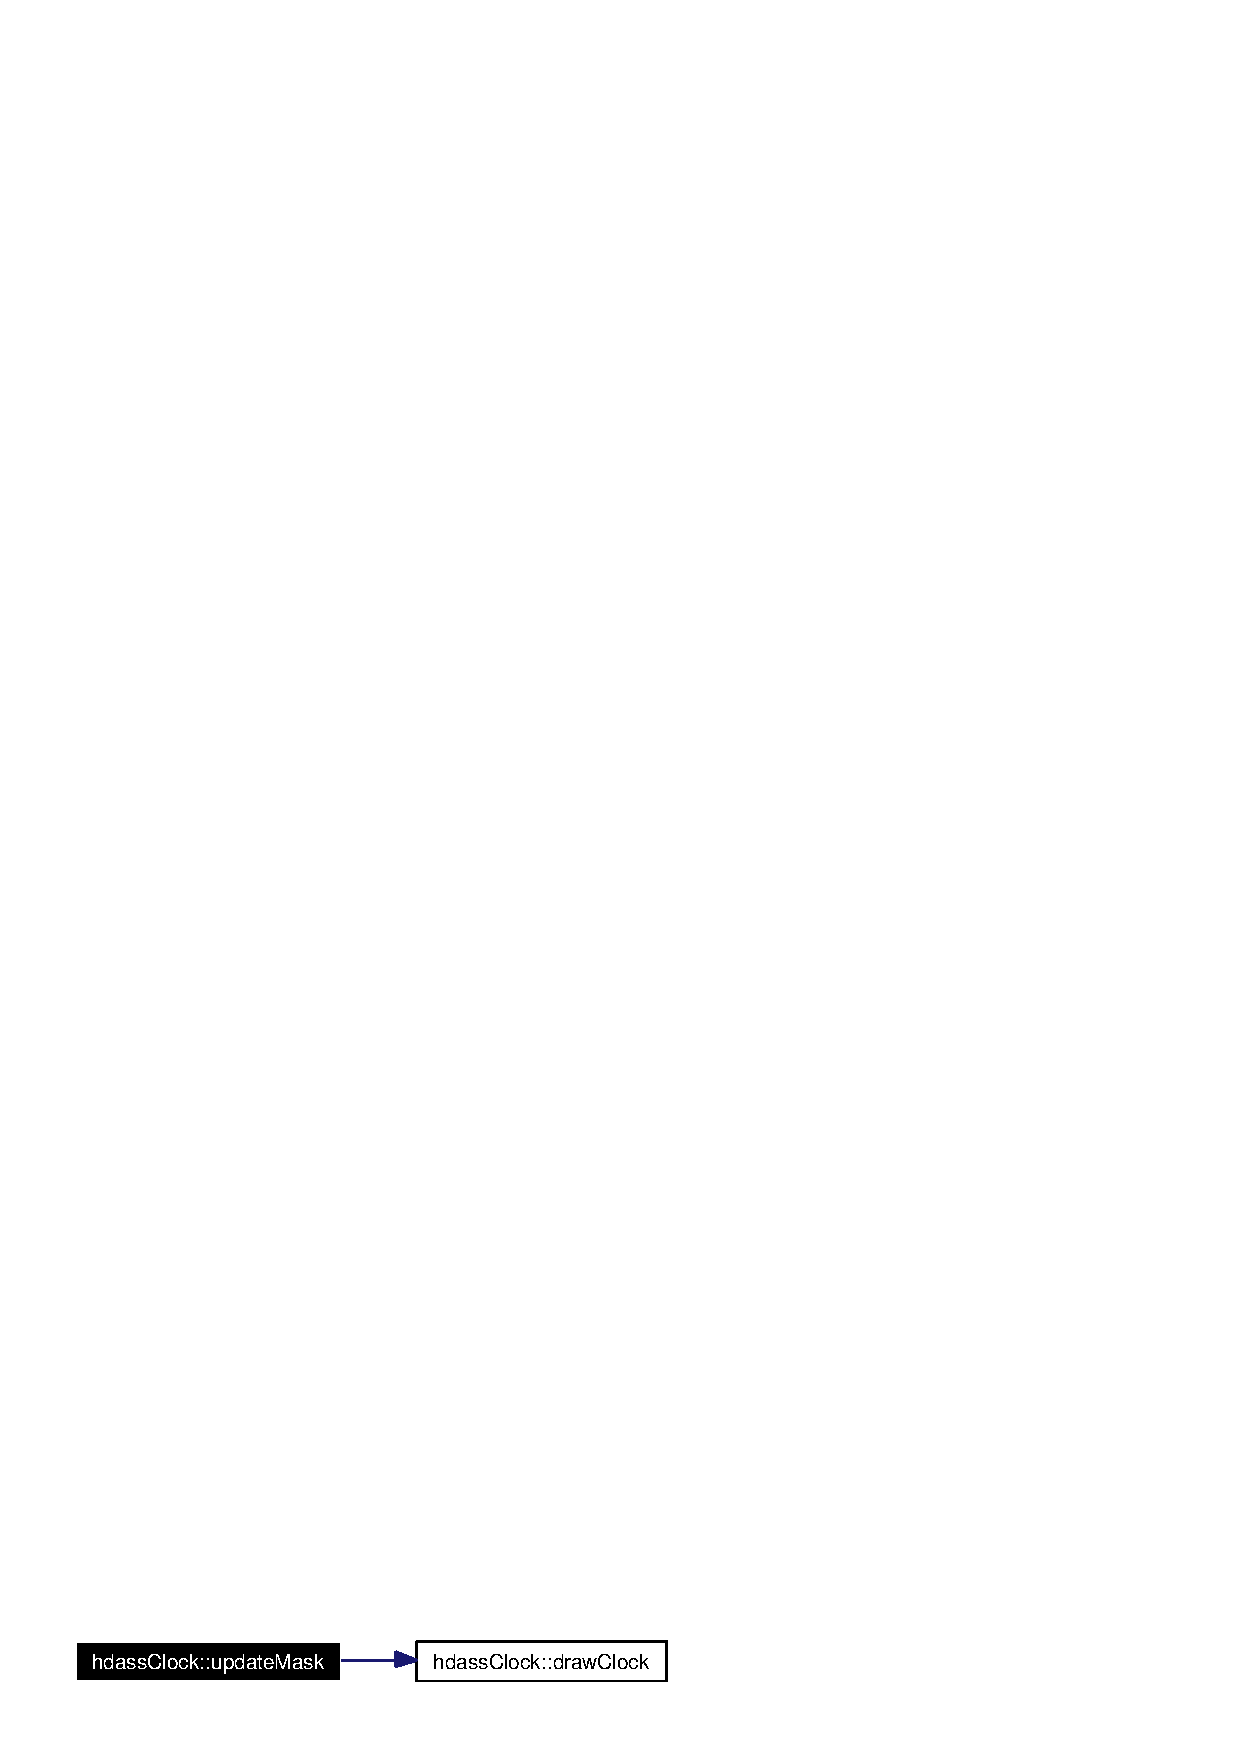
\includegraphics[width=160pt]{classhdassClock_hdassClockb0_cgraph}
\end{center}
\end{figure}
\index{hdassClock@{hdass\-Clock}!xSetup@{xSetup}}
\index{xSetup@{xSetup}!hdassClock@{hdass\-Clock}}
\subsubsection{\setlength{\rightskip}{0pt plus 5cm}void hdass\-Clock::x\-Setup ()}\label{classhdassClock_hdassClocka1}




Definition at line 36 of file hdassclock.cpp.

References internal\-Timer, time, and timeout().

Referenced by hdass\-Clock().



\footnotesize\begin{verbatim}37 {
38     time = QTime::currentTime();                // get current time
39     internalTimer = new QTimer( this ); // create internal timer
40     connect( internalTimer, SIGNAL(timeout()), SLOT(timeout()) );
41     internalTimer->start( 5000 );               // emit signal every 5 seconds
42     
43     //DAVID Setbackgorund
44     pixBackground.load("/root/kde_application/hdass08/skin/ClockBackground.png");
45     setBackgroundPixmap(pixBackground);
46     
47 }
\end{verbatim}\normalsize 


\subsection{Member Data Documentation}
\index{hdassClock@{hdass\-Clock}!clickPos@{clickPos}}
\index{clickPos@{clickPos}!hdassClock@{hdass\-Clock}}
\subsubsection{\setlength{\rightskip}{0pt plus 5cm}QPoint {\bf hdass\-Clock::click\-Pos}\hspace{0.3cm}{\tt  [private]}}\label{classhdassClock_hdassClockr0}




Definition at line 53 of file hdassclock.h.\index{hdassClock@{hdass\-Clock}!internalTimer@{internalTimer}}
\index{internalTimer@{internalTimer}!hdassClock@{hdass\-Clock}}
\subsubsection{\setlength{\rightskip}{0pt plus 5cm}QTimer$\ast$ {\bf hdass\-Clock::internal\-Timer}\hspace{0.3cm}{\tt  [private]}}\label{classhdassClock_hdassClockr2}




Definition at line 55 of file hdassclock.h.

Referenced by set\-Time(), and x\-Setup().\index{hdassClock@{hdass\-Clock}!pixBackground@{pixBackground}}
\index{pixBackground@{pixBackground}!hdassClock@{hdass\-Clock}}
\subsubsection{\setlength{\rightskip}{0pt plus 5cm}QPixmap {\bf hdass\-Clock::pix\-Background}\hspace{0.3cm}{\tt  [private]}}\label{classhdassClock_hdassClockr3}




Definition at line 56 of file hdassclock.h.\index{hdassClock@{hdass\-Clock}!time@{time}}
\index{time@{time}!hdassClock@{hdass\-Clock}}
\subsubsection{\setlength{\rightskip}{0pt plus 5cm}QTime {\bf hdass\-Clock::time}\hspace{0.3cm}{\tt  [private]}}\label{classhdassClock_hdassClockr1}




Definition at line 54 of file hdassclock.h.

Referenced by draw\-Clock(), set\-Time(), timeout(), and x\-Setup().

The documentation for this class was generated from the following files:\begin{CompactItemize}
\item 
{\bf hdassclock.h}\item 
{\bf hdassclock.cpp}\end{CompactItemize}
